\chapter{Results Overview}
This study provides several results that can be divided into two categories:
\vspace{-5mm}
\begin{itemize}
 \setlength{\itemsep}{-5pt} 
\item Implemented Python Systems
\item Generated evidences and values
\end{itemize}

Furthermore, since a significant amount of time and effort was spend for setting up the datasets, it's possible to consider them like results as well.\\
If you're interested to check out the whole results and even reuse it, it's possible to find it on the already cited Github repository\footnote{System repository: https://github.com/Sprea22/Python\_Systems}. 

\section{Implemented Python Systems}
\vspace{-5mm}
\begin{itemize}
 \setlength{\itemsep}{-5pt} 
\item \textbf{SIA.py} : System able to provide an initial analysis and displaying about a specific dataset's parameter dataset.
\item \textbf{MIA.py} : System able to provide an initial analysis and displaying about all the parameters of a specific dataset.
\item \textbf{Map.py} : System able to provide an initial cartographic visualization about a specific parameter in the Norwegian territory.
\item \textbf{ARIMA-Evaluate.py} : System able to provide an evaluation about different configurations of an ARIMA machine, appplied to a specific dataset's parameter.
\item \textbf{ARIMA-Future.py} : System able to calculate and display some future values prediction and compare it with the real values (if available) using the ARIMA model.
\end{itemize}

\newpage

\section{Generated Evidences and values}
\textbf{Analysis Results} - For each dataset have been provided:
\vspace{-5mm}
\begin{itemize}
 \item Document containing the correlation coefficients between all the dataset parameters and the corresponding correlation matrix graphic.
 \item Graphic displaying and comparing the normalized angular coefficients of all the dataset paramaters.
 \item For each single parameter of the the dataset:
\begin{itemize}
\item Total graphic and trend line of the dataset values.
\item Graphic displaying the different years plot.
\item Document containing the correlation coefficients values between different years and the corresponding correlation matrix graphic.
\item Document containing the correlation coefficients values between different months and the corresponding correlation matrix graphic.
\item Document containing the angular coefficient and the normalized angular coefficients of the trend line.
\end{itemize}
\end{itemize}

\textbf{Forecast Results} - The Evaluation and Future prediction systems have been executed just on the most interesting parameter of some dataset, due to the short time left and to the Evaluation procedure that takes a lot of time. More in particular, it's possible to check out the Evaluation MAPE Results, Preditcted future values results and Real future values about the parameter "Feed Consumption" for the following counties: Finnmark, Troms, Nordland, Hordaland and whole Norway,

\textbf{Map Results} - Contains several results about the map system. In particular different cartographic map about Norway with different average inputs on a range of time between 2007 and 2014.
		
\section{Particularly interesting results}
In the following two pages is reported a small portion of the results written above. \\
The reason for this choice is that they will be indispensable for the discussion during the next chapter. \\
The list of figures [\ref{fig: Norway_feed}, \ref{fig: Finnmark_feed}, \ref{fig: Troms_feed}, \ref{fig: Nordland_feed}, \ref{fig: Hordaland_feed}] shows the values shape for each year of some specific datasets (Norway, Finnmark, Troms, Nordland, Hordaland).\\
The table \ref{table: RealPredMAPE1} and \ref{table: RealPredMAPE2} show some specific results of the Forecast System.

\newpage

\vspace{-5mm}
\makebox[1\textwidth][c]{
\begin{minipage}[t]{0.7\textwidth}
\begin{figure}[H]
    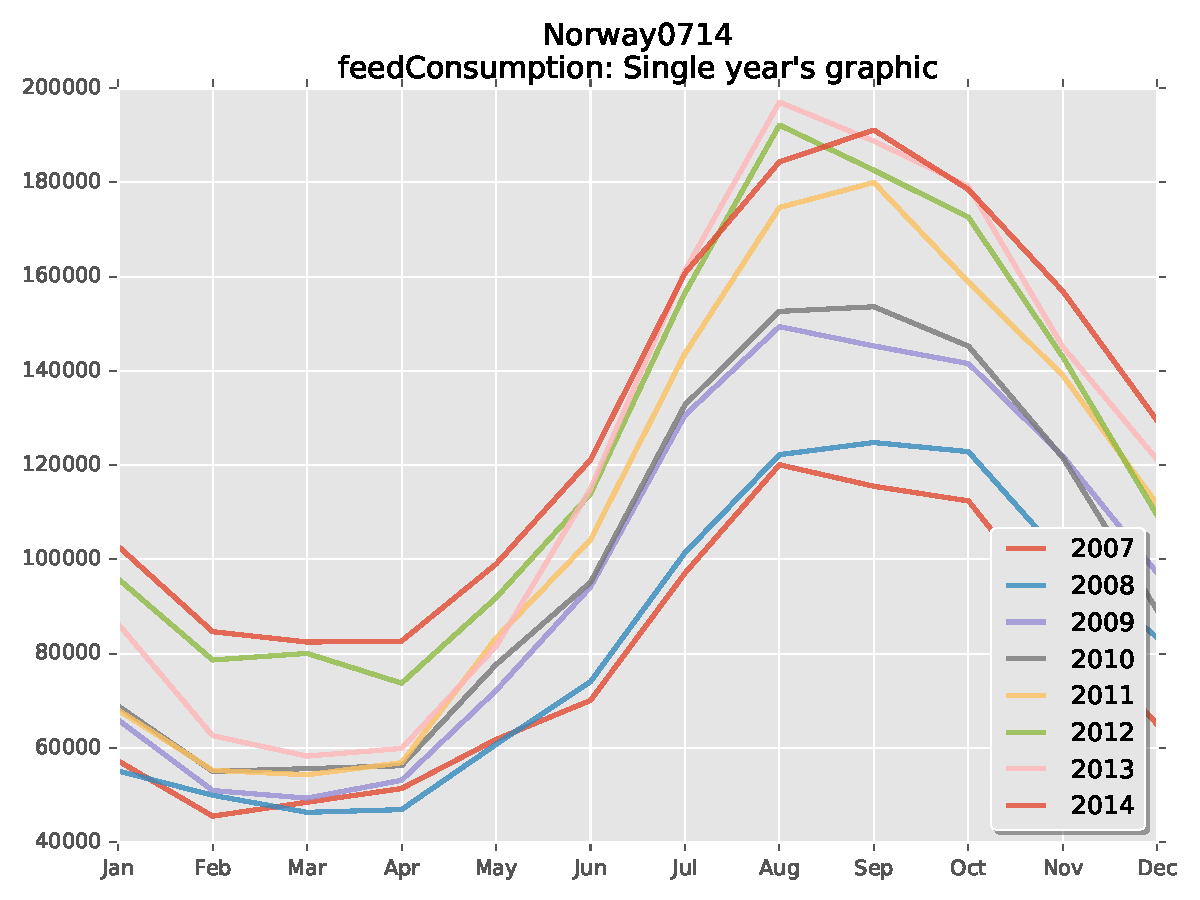
\includegraphics[trim={0 0 0 0},clip,width=1\textwidth]{Files/Norway0714_feedConsumption_years.pdf}
    \caption{Annual consumption of feed trend in Norway. }
    \label{fig: Norway_feed}
\end{figure}
\end{minipage}}

\makebox[1\textwidth][c]{
\begin{minipage}[t]{0.5\textwidth}
\begin{figure}[H]
    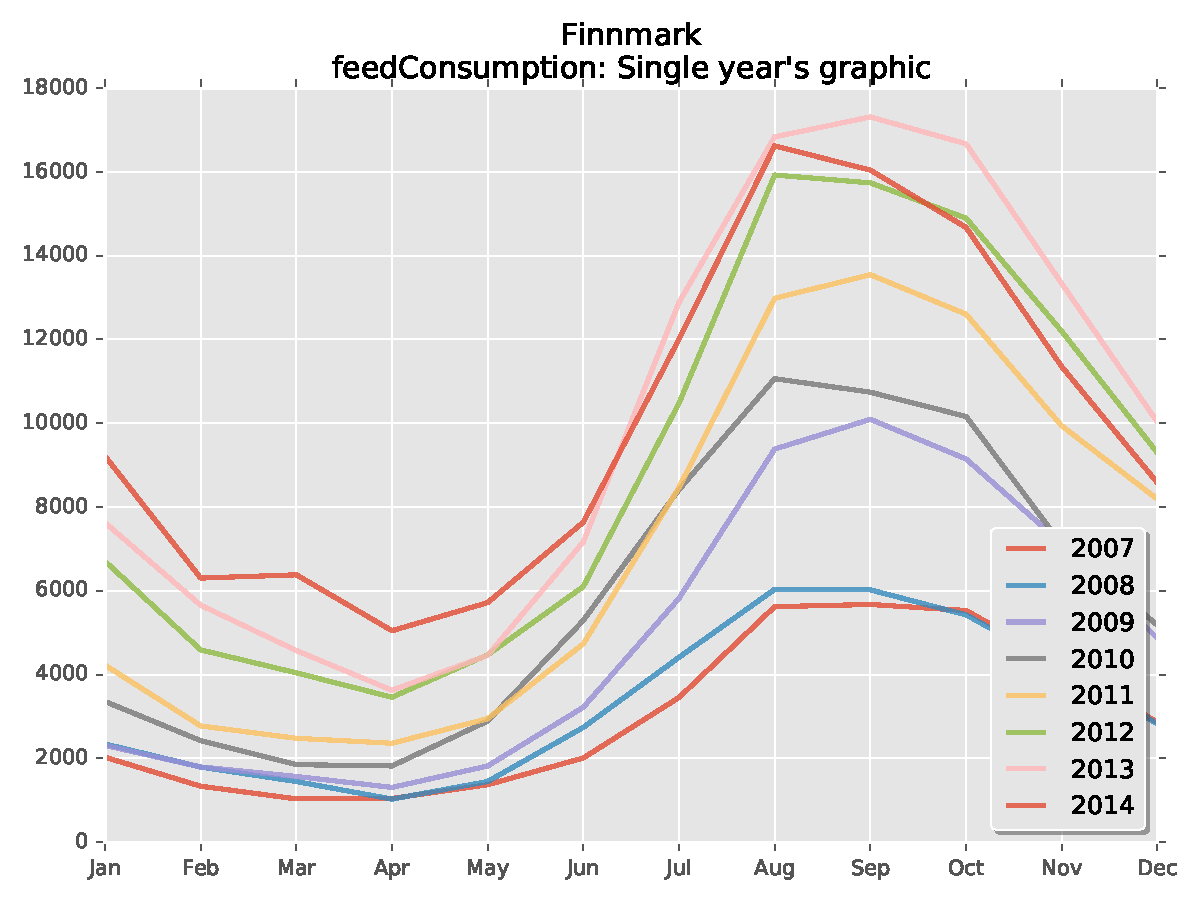
\includegraphics[trim={0 0 0 0},clip,width=1\textwidth]{Files/Finnmark_feedConsumption_years.pdf}
    \caption{Annual consumption of feed trend in Finnmark. }
    \label{fig: Finnmark_feed}
\end{figure}
\end{minipage} \hfill
\begin{minipage}[t]{0.5\textwidth}
\begin{figure}[H]
    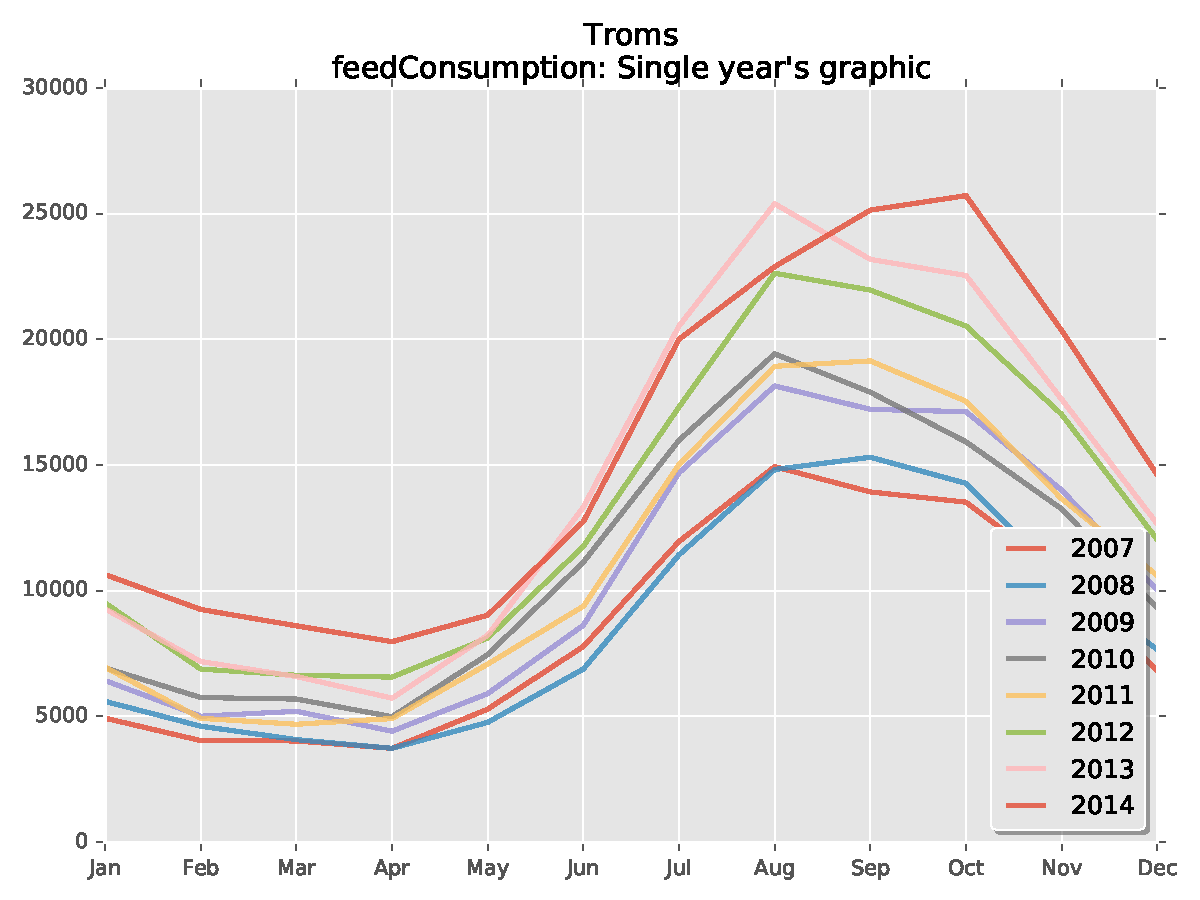
\includegraphics[trim={0 0 0 0},clip,width=1\textwidth]{Files/Troms_feedConsumption_years.pdf}
    \caption{Annual consumption of feed trend in Troms. }
    \label{fig: Troms_feed}
\end{figure}
\end{minipage}}


\makebox[1\textwidth][c]{
\begin{minipage}[t]{0.5\textwidth}
\begin{figure}[H]
    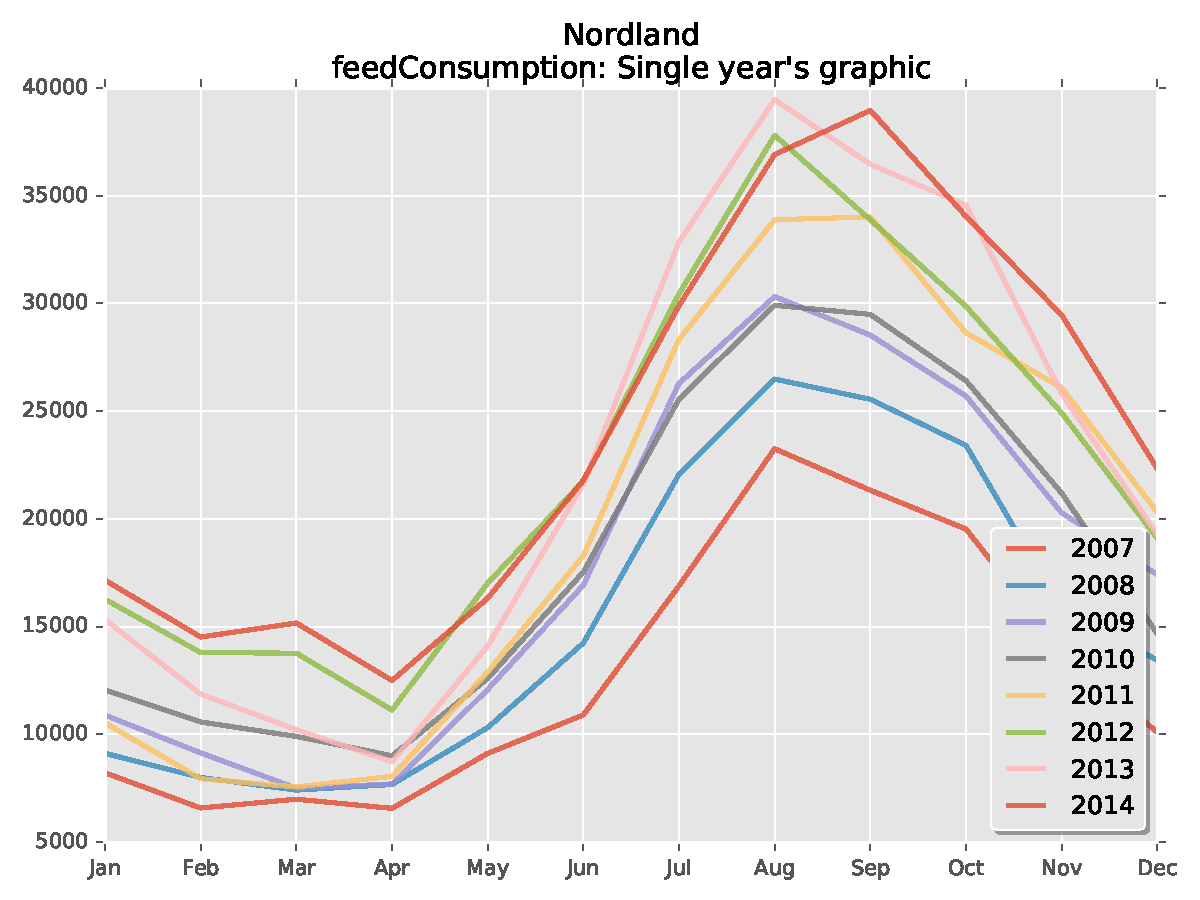
\includegraphics[trim={0 0 0 0},clip,width=1\textwidth]{Files/Nordland_feedConsumption_years.pdf}
    \caption{Annual consumption of feed trend in Nordland. }
    \label{fig: Nordland_feed}
\end{figure}
\end{minipage} \hfill
\begin{minipage}[t]{0.5\textwidth}
\begin{figure}[H]
    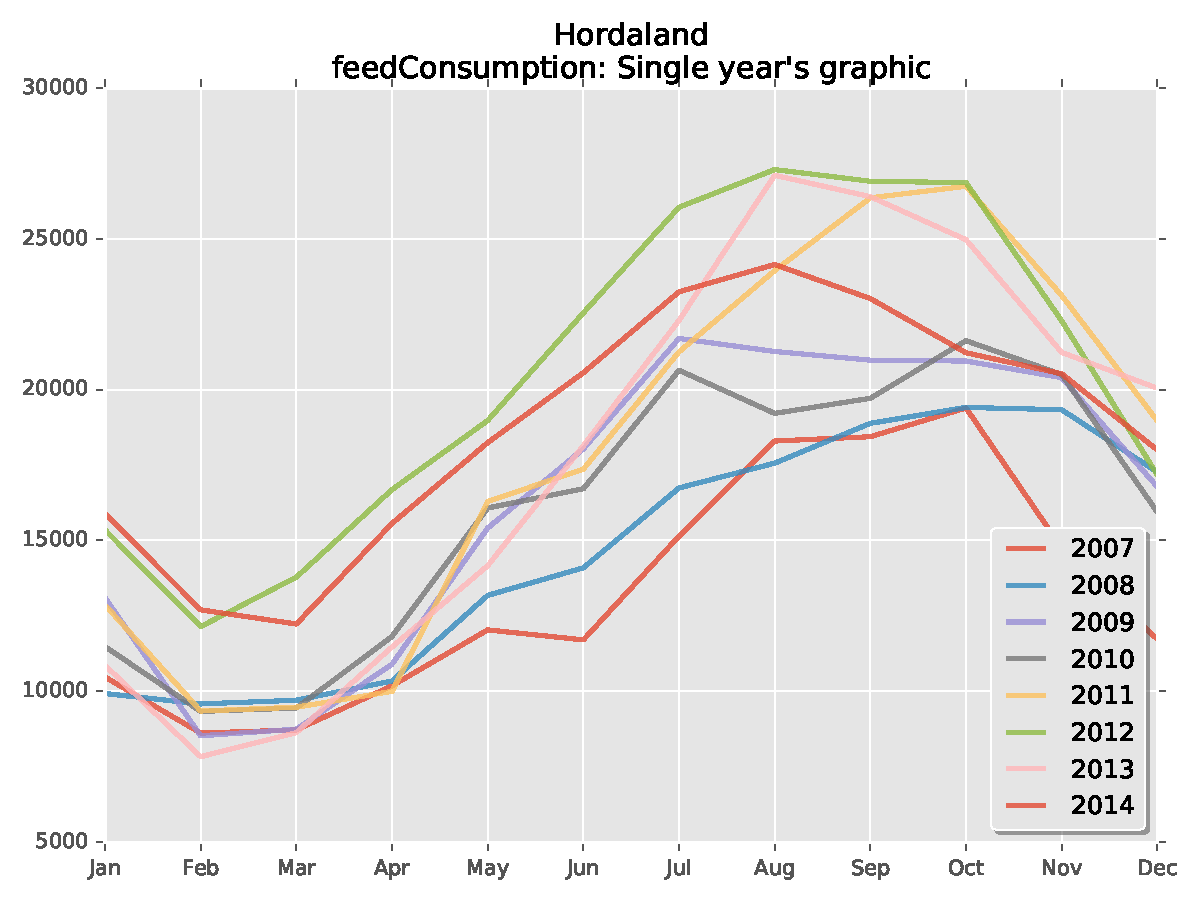
\includegraphics[trim={0 0 0 0},clip,width=1\textwidth]{Files/Hordaland_feedConsumption_years.pdf}
    \caption{Annual consumption of feed trend in Hordaland. }
    \label{fig: Hordaland_feed}
\end{figure}
\end{minipage}}

\newpage

The table [\ref{table: RealPredMAPE1}] shows the Prediction results about the parameter "Feed Consumption" of the dataset "Norway".  In particular are reported:
\vspace{-5mm}
\begin{itemize}
 \setlength{\itemsep}{-5pt} 
 \item ARIMA order used for the predictions (just on the right of the dataset name).
 \item Real 2015 consumption of feed values. 
 \item Predicted 2015 consumption of feed values.
 \item MAPE between real and predicted values.
\end{itemize}

The Prediction results have been reported for some of the Norwegian counties, such as:\\
Finnmark and Hordaland in the table [\ref{table: RealPredMAPE2}]. \\ Nordland and Troms in the table [\ref{table: RealPredMAPE3}].


\vspace{+15mm}


\begin{table}[ht]
\makebox[\textwidth][c]{
\begin{tabular}{|c|c|c|c|c|c|}
\hline
\multirow{3}{*}{\textbf{Pred Months}} & \multicolumn{3}{c|}{\textbf{Norway : (6, 1, 0)}} \\
\cline{2-4}
 & \textbf{Real} & \textbf{Pred} & \textbf{Error} \\
\hline
 January 2015 &  109459 & 101149.42 & 7.59\%  \\
\hline
 February 2015 &  86701.5	& 83164.98 & 4.08\%   \\
 \hline
 March 2015 & 87614.3 &	78983.87 &	9.85\%   \\
 \hline
 April 2015 & 84920.3 &	91419.33 &	7.65\%   \\
 \hline
 May 2015 & 94545.2 &	114388.79 &	20.99\% 	\\
 \hline
 June 2015 & 112220 &	141620.77 &	26.20\%  \\
 \hline
 July 2015 & 152023 &	166470.71 &	9.50\%   \\
 \hline
 August 2015 & 186931 &	181705.78 &	2.80\% \\
 \hline
 September 2015 & 181735 & 184349.66 &	1.44\%  \\
 \hline
 October 2015 &  177401 &	173328.08 & 2.30\%  \\
 \hline
 November 2015 &  153730 &	152941.90 &	0.51\%  \\
 \hline
 December 2015 & 126324 & 129326.56 & 2.38\%  \\
 \hline
\end{tabular}  }
    \caption[Norway: Predicted feed consumption values: Real, Pred, Error. ]{Comparison between real 2015 "feed consumption" values and their prediction, with the corresponding MAPE for the counties: Norway}
    \label{table: RealPredMAPE1}
\end{table}

\newpage

\begin{table}[ht]
\makebox[\textwidth][c]{
\resizebox{1\textwidth}{!}{
\begin{tabular}{|c|c|c|c|c|c|c|c|c|}
\hline
\multirow{3}{*}{\textbf{Pred Months}} & \multicolumn{3}{c|}{\textbf{Finnmark : (6,1,0)}} & \multicolumn{3}{c|}{\textbf{Hordaland : (8, 0, 0)}} \\
\cline{2-7}
 & \textbf{Real} & \textbf{Pred} & \textbf{Error} & \textbf{Real} & \textbf{Pred} & \textbf{Error} \\
\hline 
 January 2015 & 7571.038 	& 	6902.50 & 8.83 \% 		& 15039.948 & 16199.46	 & 7.71\%  \\
\hline
 February 2015 & 4947.371 	& 	4892.92 & 1.10\% 		& 12432.481 & 14638.11	 & 17.74\%  \\
 \hline
 March 2015 & 4686.465 		& 5171.14	& 10.34\% 		& 12523.293 & 14596.72	 & 16.56\% \\
 \hline
 April 2015 & 4263.749		 & 	6309.80 & 47.99\%		& 14231.265 & 15673.42	 & 10.13\%  \\
 \hline
 May 2015 & 5472.568 		& 8927.99	& 63.14\%		& 14543.612 & 17305.97	 & 18.99\% \\
 \hline
 June 2015 & 8270.913 		& 11867.40 & 43.48\%		& 15314.691 & 18694.21	 & 22.07\% \\
 \hline
 July 2015 & 12356.162 		& 13499.17	& 9.25\%		& 19617.51 & 19996.28	 & 1.93\%   \\
 \hline
 August 2015 & 15877.981 	& 	14484.53 & 8.78\%		& 26429.183 & 20583.11 & 22.12\% \\
 \hline
 September 2015 & 15382.371 & 13848.08	& 9.97\%		& 28152.314 & 20524.85 & 27.09\%  \\
 \hline
 October 2015 & 15039.109 	& 12583.28	& 16.33\%		& 26869.594 & 19565.15	 & 27.18\% \\
 \hline
 November 2015 & 11453.453 	& 	10842.37 & 5.34\%		& 23914.498 & 18086.76 & 24.37\%  \\
 \hline
 December 2015 & 9450.334 	& 8898.79	 & 5.84\%		& 20332.347 & 16519.30	 & 18.75\%  \\
 \hline
\end{tabular}  }}
    \caption[Finnmark, Hordaland: Predicted feed consumption values: Real, Pred, Error. ]{Comparison between real 2015 "feed consumption" values and their prediction, with the corresponding MAPE for the counties: Finnmark, Hordaland}
    \label{table: RealPredMAPE2}
\end{table}

\vspace{+15mm}

\begin{table}[ht]
\makebox[\textwidth][c]{
\begin{tabular}{|c|c|c|c|c|c|c|c|c|}
\hline
\multirow{3}{*}{\textbf{Pred Months}} & \multicolumn{3}{c|}{\textbf{Nordland : (6, 0, 0)}} & \multicolumn{3}{c|}{\textbf{Troms : (2, 0, 0)}} \\
\cline{2-7}
 & \textbf{Real} & \textbf{Pred} & \textbf{Error} & \textbf{Real} & \textbf{Pred} & \textbf{Error} \\
\hline
 January 2015 & 20077.7	& 16178.44 &	19.42\% 				&  12534.708		& 9024.37	 & 28.00\%  \\
\hline
 February 2015 &  	15478.6 &	11811.61 &	23.69\% 			&  9098.07		& 4915.31	 & 45.97\%  \\
 \hline
 March 2015 & 15477.5 & 9251.12	& 40.23 \% 						&  9381.861		& 	3017.57 & 67.84\% \\
 \hline
 April 2015 &	12938.3 &	9571.32 &	26.02\%					& 9493.93		& 3431.09	& 63.86\%    \\
 \hline
 May 2015 &  15237.5 &	11685.79 &	23.31\%						&	11215.47	& 5691.14	 & 49.26\%  	\\
 \hline
 June 2015 & 20228.9 &	15136.22 &	25.18\%						& 16370.732		& 8968.26	 & 45.22\%  \\
 \hline
 July 2015 & 29049.6 &	18922.35 &	34.86\%						& 21041.845		& 12323.02	 & 41.44\%   \\
 \hline
 August 2015 &  37051.1	& 22044.15	& 40.50\%					& 26981.845		& 14946.55	 & 44.61\% \\
 \hline
 September 2015 &  35364.5 & 24037.46 & 32.03\%					& 25229.126		&  16331.88	& 35.27\%  \\
 \hline
 October 2015 & 33985.7 & 24545.52 & 27.78\%					& 27327.632		&  16346.43 &  40.18\%   \\
 \hline
 November 2015 &  28439.4 &	23736.48 &	16.54\%					& 22476.374		& 15204.13 	& 32.36\%  \\
 \hline
 December 2015 & 21447.6 & 22001.57 & 2.58\%					& 17239.549		& 13359.68	 & 22.51 \%  \\
 \hline
\end{tabular}  }
    \caption[Nordland, Troms: Predicted feed consumption values: Real, Pred, Error. ]{Comparison between real 2015 "feed consumption" values and their prediction, with the corresponding MAPE for the counties: Nordland, Troms}
    \label{table: RealPredMAPE3}
\end{table}

